% Analysis conditions of the two-cylinder quarter model
% (two long cylinders between rigid plates, quarter model with symmetry BCs)
% Standard structural-analysis symbols drawn in plain TikZ:
%   roller supports (triangle + circles + hatched ground) for the symmetry
%   wall and the supported edge, hatched rigid plate with the nodal force.
\documentclass[border=8pt]{standalone}
\usepackage{tikz}
\usetikzlibrary{arrows.meta,decorations.markings,patterns.meta}

% roller support: triangle tip at #1, base away from the contact plane,
% rotated so that it blocks the normal direction of the surface
\newcommand{\rollersym}[3]{% #1 = x, #2 = y (tip), #3 = rotation
  \begin{scope}[shift={(#1,#2)}, rotate=#3]
    \draw[fill=white] (0,0) -- (-0.09,0.16) -- (0.09,0.16) -- cycle;
    \draw[fill=white] (-0.075,0.20) circle (0.022);
    \draw[fill=white] (0.075,0.20) circle (0.022);
    \draw (-0.11,0.235) -- (0.11,0.235);
    \draw[gray] (-0.13,0.245) -- (-0.10,0.285);
    \draw[gray] (-0.06,0.245) -- (-0.03,0.285);
    \draw[gray] (0.01,0.245) -- (0.04,0.285);
    \draw[gray] (0.08,0.245) -- (0.11,0.285);
  \end{scope}
}

\begin{document}
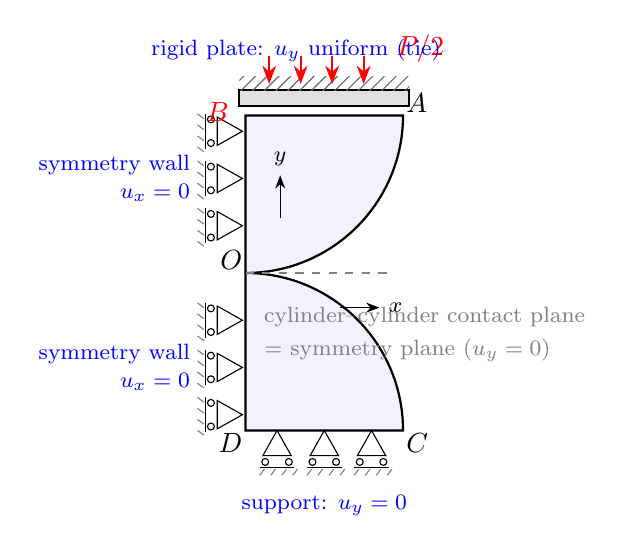
\begin{tikzpicture}[>={Stealth}, scale=2.0]

  % ================= quarter model geometry =================
  % upper lobe: quarter disk centered B(0,1); lower lobe: centered D(0,-1)
  \coordinate (O) at (0,0);
  \coordinate (B) at (0,1);
  \coordinate (A) at (1,1);
  \coordinate (C) at (1,-1);
  \coordinate (D) at (0,-1);

  \draw[thick, fill=blue!5]
    (B) -- (A) arc[start angle=0, end angle=-90, radius=1] % A -> O
    arc[start angle=90, end angle=0, radius=1]             % O -> C
    -- (D) -- cycle;

  % ================= symmetry wall: rollers (u_x = 0, free u_y) =========
  \rollersym{-0.02}{0.30}{90}
  \rollersym{-0.02}{0.60}{90}
  \rollersym{-0.02}{0.90}{90}
  \rollersym{-0.02}{-0.30}{90}
  \rollersym{-0.02}{-0.60}{90}
  \rollersym{-0.02}{-0.90}{90}
  \node[left, blue, inner sep=4pt, align=right] at (-0.28, 0.6)
    {\footnotesize symmetry wall\\[-2pt]\footnotesize $u_x=0$};
  \node[left, blue, inner sep=4pt, align=right] at (-0.28, -0.6)
    {\footnotesize symmetry wall\\[-2pt]\footnotesize $u_x=0$};

  % ================= rollers under CD (u_y = 0) =================
  \rollersym{0.20}{-1.0}{180}
  \rollersym{0.50}{-1.0}{180}
  \rollersym{0.80}{-1.0}{180}
  \node[below, blue, inner sep=4pt] at (0.5, -1.34)
    {\footnotesize support: $u_y=0$};

  % ================= rigid plate above AB (uniform u_y) =================
  \draw[thick, fill=black!12] (-0.04, 1.06) rectangle (1.04, 1.16);
  \fill[pattern={Lines[angle=45, distance=3pt]}, pattern color=black!60]
    (-0.04, 1.16) rectangle (1.04, 1.25);
  \foreach \x in {0.15, 0.35, 0.55, 0.75} {
    \draw[red, thick, ->] (\x, 1.38) -- (\x, 1.20);
  }
  \node[above right, red, inner sep=2pt] at (0.92, 1.3) {$P/2$};
  \node[above, blue, inner sep=4pt] at (0.32, 1.27)
    {\footnotesize rigid plate: $u_y$ uniform (tie)};

  % ================= contact plane annotation =================
  \draw[dashed, gray] (O) -- (0.9, 0);
  \node[below right, gray, inner sep=2pt, align=left] at (0.08, -0.18)
    {\footnotesize cylinder--cylinder contact plane\\
     \footnotesize $=$ symmetry plane ($u_y=0$)};

  % ================= node labels =================
  \node[left, red, inner sep=3pt] at (-0.05, 1.02) {$B$};
  \node[above right, inner sep=1pt] at (A) {$A$};
  \node[below right, inner sep=1pt] at (C) {$C$};
  \node[below left, inner sep=1pt] at (D) {$D$};
  \node[above left, inner sep=1pt] at (O) {$O$};

  % ================= axes =================
  \draw[->] (0.60, -0.22) -- (0.85, -0.22) node[right] {\footnotesize $x$};
  \draw[->] (0.22, 0.35) -- (0.22, 0.62) node[above] {\footnotesize $y$};

\end{tikzpicture}
\end{document}
